\documentclass{article}
\usepackage{fixltx2e}
\usepackage{float}
\usepackage{amsmath}
\newcommand{\degree}{\ensuremath{^\circ}}
\usepackage{graphicx}
\usepackage[margin=1.0in]{geometry}



\title{Partial Equilibrium in Mathematica}
\author{Michael Lee, The University of Texas at Austin}

\begin{document}
\maketitle{}

Much of microeconomic analysis is based on the concept of a partial equilibrium. By using computational tools-- such as Mathematica-- we can quickly derive, plot and adapt analytical models of consumer and firm behaviour, and how the intersection of the two fix market equilibrium. 

\newpage

\section{Utility and Production Functions}

The basis of all economic analysis is the consumer and their goal of utility-maximization. The most common numerical repersentation of two-input production and consumer utility are the Cobb-Douglas and Leontief functions. These forms satisfy the following properties depending on if they are used to repersent production or utility, respectively:

\begin{center}
	\begin{enumerate}
		\item monotonicly increasing/decreasing
		\item concave/convex
		\item nonintersecting
	\end{enumerate}
\end{center}

The general Cobb-Douglas function takes the form
\begin{equation}
	Y = L^{\beta}K^{\alpha}
\end{equation}

Where \emph{Y} is production, \emph{L} is labor, \emph{K} is capital, and $\alpha , \beta$ are the elasticities of labor and capital respectively. The Cobb-Douglass ({\bf Figure 1}) function assumes that continous substitution between goods x\textsubscript{1} and x\textsubscript{2} in production/utility.

\begin{figure}[!ht]
\begin{center}
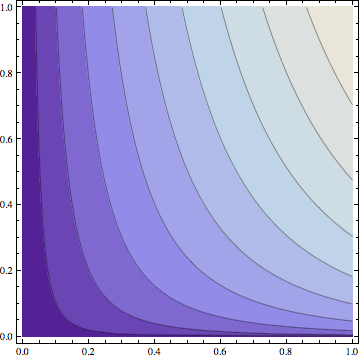
\includegraphics[scale=.5]{Figures/CobbDouglas}
\caption{A Cobb-Douglas Production Function ($\rho = .7$)}
\end{center}
\end{figure}

\begin{equation}
	\alpha + \beta = 1
\end{equation}

The above equation implies a special conditon when the production function experinces constant returns to scale. \\*
Cobb-Douglas production is a special case of the constant elasticity of substitution (CES) production function as described by Solow (Solow, 1956) when $\lim{\gamma \to 0}$. The two-factor CES function ({\bf Figure 2}) is of the form:

\begin{equation}
	Y = \alpha K^{\gamma} + (1-\alpha) L^{\gamma})^{\frac{1}{\gamma}}
\end{equation}

\begin{figure}[!ht]
	\begin{center}
	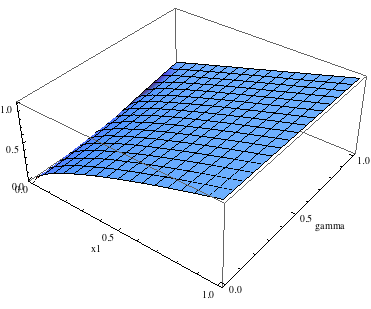
\includegraphics[scale=0.5]{Figures/CES.png}
	\caption{CES Function ($\gamma = [.01,1], x_{1} = [0,1], x_{2} = 1 $)}
	\end{center}
\end{figure}

\*

A Leontief function is a special case of a Cobb-Douglas function in which there is no substitutability between goods x\textsubscript{1} and x\textsubscript{2} and thus there exists a predefined proportion of goods x\textsubscript{1} and x\textsubscript{2} used in the production of \emph{Y}. 

\begin{equation}
	Y(x_{1}, x_2) = min(c_{1}x_{1}, c_{2}x_{2})
\end{equation}

When the proportion 
$$\frac{c_{1}x_{1}}{c_{2}x_{2}} = 1$$
the Leontief has a 45\degree line through the contour plot as seen in {\bf Figure 3}:

\begin{figure}[!ht]
	\begin{center}
	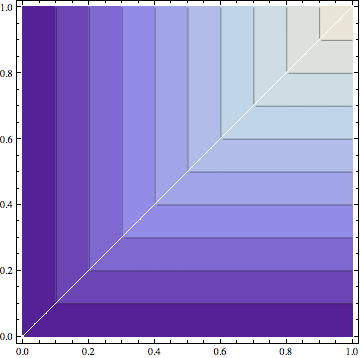
\includegraphics[scale=0.5]{Figures/Leontief.png}
	\caption{A Leontief Production Function}
	\end{center}
\end{figure}


\section{Consumer Theory}
Traditionally, consumer theory is modeled as agents maximizing their utility (strictly a function of consumption, \emph{C}) subject to their budget constraint, (\emph{m}). This implies that given some bundle of goods $x_{1}, x_{2}$ at prices $p_{1}, p_{2}$, the rational consumer will purchase the bundle that maximizes their total utility, \emph{U}. The optimal bundle will allways include an nonzero amount of both goods since utility is subject to the principle of diminishing marginal returns. \*
A Cobb-Douglas utlilty function with elasticities $\alpha$ will take the form:

\begin{align}
	max: U = x_{1}^{\alpha} x_{2}^{1-\alpha} \\
	subject to: m = p_{1}x_{1} + p_{2}x_{2}
\end{align}
\\* \\*
Via logarithims, this equation is equivelent to:

\begin{equation}
	log(U) =  \alpha log(x_{1}) + (1-\alpha) log(x_{2}) 
\end{equation}

To find the optimal bundle of goods, the Lagrangian of the system of equations is modeled in \emph{Mathematica}. The Lagrangian, $\mathcal{L}$ is written as follows:

\begin{equation}
	\mathcal{L}(x_{1}, x_{2},\lambda) = \alpha log(x_{1}) + (1-\alpha) log(x_{2}) +\lambda (m - p_{1}x_{1} -p_{2}x_{2})
\end{equation}

The partial derivative of the Lagrangian with respect to each variable is taken and set equal to zero.

\begin{align}
		\frac{d\mathcal{L}}{dx_{1}} = -p_{1}\lambda + \frac{\alpha}{x_{1}} ==0 \\
		\frac{d\mathcal{L}}{dx_{2}} = -p_{2}\lambda + \frac{1-\alpha}{x_{2}} ==0 \\
		\frac{d\mathcal{L}}{dx_{\lambda}} = m - p_{1}x_{1} - p_{2}x_{2} == 0
\end{align}


This system of equations can be solved for the demand curves of $x_{1}$ and $x_{2}$, the results of which are plotted below. 

\begin{figure}[!ht]
	\begin{center}
	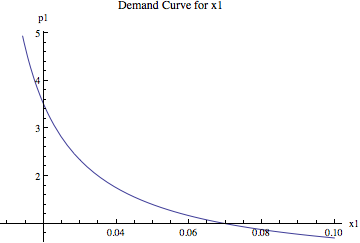
\includegraphics[scale=.75]{Figures/x1Demand}
	\caption{Consumer Demand Function, $x_{1}$ vs $p_{1}$}
	\end{center}
\end{figure}


\section{Firms}
In opposition to consumers goal of utilitiy-maximization, firms are modeled as stictly profit-maximizing entities. In the original model, the firm's profit-maximization function is expressed mathematically as:


\begin{align}
	max: \pi = p_{1}x_{1} - wL \\ 
	subject to: x_{1} = TL^{\beta}
\end{align}


Where \emph{w} are wages, \emph{L} is labor supply, \emph{T} is the given technology level, and $\beta$ is the production's elasticity to labor. By substituting the profit function $\pi$ into the production function and setting the resulting function's derivative with respect to labor (\emph{L}) to zero, we establish the labor demand function. 

\begin{equation}
	L = \frac{w}{\beta p_{1} T})^{\frac{1}{-1+\beta}}
\end{equation}

\begin{figure}[!ht]
	\begin{center}
	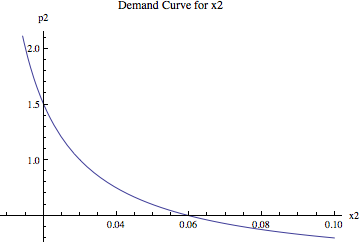
\includegraphics[scale=.75]{Figures/LaborDemand}
	\caption{Labor Demand Curve ($\beta = .4$, T = 1, $p_{1}= 1$)}
	\end{center}
\end{figure}

Substituting the labor demand function ({\bf 6}) into the production function ({\bf 13}) we find the supply curve. 

\begin{equation}
	S = T[(\frac{w}{\beta p_{1} T})^{\frac{1}{-1+\beta}}]^{\beta}
\end{equation}

\begin{figure}[!ht]
	\begin{center}
	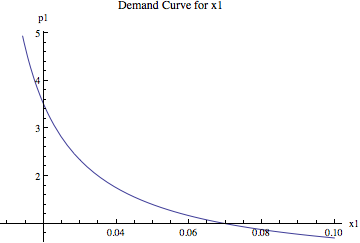
\includegraphics[scale=.75]{Figures/Supply}
	\caption{Supply Curve for $x_{1}$  ($\beta = .4$, T = 1, w = 100)}
	\end{center}
\end{figure}

\newpage

\section{Market Equilibrium}
Using the supply and demand curves established earlier, we can derive the equation for market equilbrium. The demand curve found in Part 2 and the supply function as described in Part 3 are set equal to one another to find market equilibrium. 

\begin{equation}
	\frac{\alpha m}{x_{1}} == w \frac{((\frac{x_{1}}{T})^{\frac{1}{\beta}})^{1-\beta}}{\beta T}
\end{equation}

In {\bf Figure 7} the effects of different levels of total factor productivity \emph{T} are shown. TFP is used as a metric of the level of how efficiently the economy can convert inputs to outputs. Historically, this factor serves mainly as a variable that can be altered in curve-fitting the model to real world data.

 \begin{figure}[!ht]
	\begin{center}
	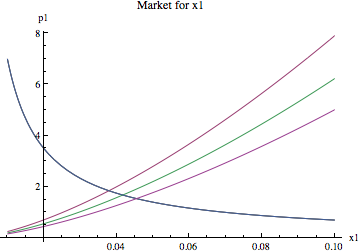
\includegraphics[scale=.75]{Figures/MarketEquilT}
	\caption{Market Equilibrium for $x_{1}$ as a function of \emph{T}}
	\end{center}
\end{figure}

The effects of changing consumer's elasticity $\alpha$ to good $x_{1}$ can be seen in {\bf Figure 8}. Higher elasticity values correspond with higher curves as consumers are less reponsive to price changes of $x{1}$

 \begin{figure}[!ht]
	\begin{center}
	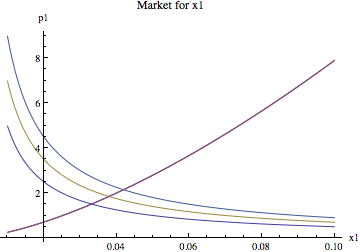
\includegraphics[scale=.75]{Figures/MarketEquilBeta}
	\caption{Market Equilibrium for $x_{1}$ as a Function on $\beta$}
	\end{center}
\end{figure}

\section{Future Improvements to the Model}

The current market equilbrium model could be improved by adding the effects of taxes. However, simply adding a flat tax would only serve to shift the results above down as the budget constraint would be reduced. To make the model more interesting, a consumption tax could be added, such that the price of good $x_{1}$ would be dependent on the amount consumed. This could be implememted using the following psuedocode:

\begin{verbatim}
\begin{center}
px1 = px1_0 + tauqx1
\end{center}
\end{verbatim}

\newpage

\section{Refrences}
Jesus Filipe and Gerard Adams (2005). 'The Estimation of the Cobb Douglas Function'. Eastern Economic Journal 31 (3): 427–445. 





\end{document}